% Chapter 4

\chapter{实证分析}
\section{Fama-MacBeth截面回归}\label{sfmb}
表~\ref{fmb}~展现了对于所有公司Fama-MacBeth的时间序列截面回归结果,对于两种方法,自左向右三列分别选用了不同的解释变量来表现错误定价因子M的预测能力,所有列均控制了行业固定效应,括号内的数字代表t值。

其中,第一列仅采用了M作为解释变量,结果非常显著;第二、三列新加入了部分公司特征:beta值、市净率BM以及三个动量因子lagretn、mom12、mom36;第四、五列加入了更多公司特征变量:市盈率EP、净经营性资产增长率grltnoa与毛利率PA,让回归更为完整,错误定价因子M同样显著,说明错误定价因子M可以用来预测股票未来收益。

%\begin{table}[htbp]\centering
%\def\sym#1{\ifmmode^{#1}\else\(^{#1}\)\fi}
%\caption{Fama-MacBeth截面回归}
%\label{fmb}
%\begin{tabular*}{\hsize}{@{\hskip\tabcolsep\extracolsep\fill}*{6}{c}}
%\toprule
%          &\multicolumn{1}{c}{(1)}&\multicolumn{1}{c}{(2)}&\multicolumn{1}{c}{(3)}&\multicolumn{1}{c}{(4)}&\multicolumn{1}{c}{(5)}\\
%          &\multicolumn{1}{c}{$R_{t+1}$}&\multicolumn{1}{c}{$R_{t+1}$}&\multicolumn{1}{c}{$R_{t+1}$}&\multicolumn{1}{c}{$R_{t+1}$}&\multicolumn{1}{c}{$R_{t+1}$}\\
%\midrule
%$M$         &    1.827\sym{***}&                  &    2.032         &                  &    20.81\sym{**} \\
%          &   (3.21)         &                  &   (1.05)         &                  &   (2.05)         \\
%$mktcap  $     &                  &   -3.819\sym{***}&   -3.733\sym{***}&    22.57         &   -3.404\sym{**} \\
%          &                  &  (-7.20)         &  (-6.63)         &   (0.82)         &  (-2.18)         \\
%$beta  $    &                  &    1.045         &    3.841\sym{**} &    19.31\sym{***}&    15.01\sym{***}\\
%          &                  &   (0.24)         &   (2.49)         &   (6.03)         &   (5.00)         \\
%$BM $       &                  &    7.675         &    13.36\sym{***}&    151.0         &   -14.60         \\
%          &                  &   (0.94)         &   (4.38)         &   (0.96)         &  (-1.49)         \\
%$lagretn $  &                  &    2.279         &    6.545\sym{***}&   -37.24         &   -3.441         \\
%          &                  &   (1.43)         &   (5.04)         &  (-0.61)         &  (-0.94)         \\
%$mom12$     &                  &    2.441         &    3.438\sym{***}&   -14.68         &    9.254\sym{***}\\
%          &                  &   (1.20)         &   (3.99)         &  (-0.73)         &   (5.12)         \\
%$mom36   $  &                  &    1.404         &    1.360\sym{*}  &   -35.65         &    8.705\sym{***}\\
%          &                  &   (1.32)         &   (1.93)         &  (-0.89)         &   (3.24)         \\
%$EP $       &                  &                  &                  &   -322.7         &    77.47         \\
%          &                  &                  &                  &  (-0.83)         &   (0.34)         \\
%$grltnoa$   &                  &                  &                  &    80.03         &    1.337         \\
%          &                  &                  &                  &   (1.11)         &   (0.24)         \\
%$PA    $    &                  &                  &                  &   -646.9         &   -65.27         \\
%          &                  &                  &                  &  (-1.27)         &  (-0.51)         \\
%行业固定效应&    控制   &    控制 &      控制   &    控制 &      控制 \\
%\midrule
%$N   $     &   87722         &    87722         &    42563         &    42563   &44659          \\
%$R^2$         &   0.0499         &    0.400         &    0.439         &    0.615         &    0.665     \\
%\bottomrule
%\multicolumn{6}{l}{\footnotesize \textit{t} statistics in parentheses}\\
%\multicolumn{6}{l}{\footnotesize \sym{*} \(p<0.1\), \sym{**} \(p<0.05\), \sym{***} \(p<0.01\)}\\
%\end{tabular*}
%\end{table}

\begin{table}[htbp]\centering
\def\sym#1{\ifmmode^{#1}\else\(^{#1}\)\fi}
\caption{Fama-MacBeth截面回归}
\label{fmb}
\begin{tabular*}{\hsize}{@{\hskip\tabcolsep\extracolsep\fill}*{7}{c}}
\toprule
&\multicolumn{3}{c}{随机森林}&\multicolumn{3}{c}{GBDT}\\
\cline{2-7} 
        &\multicolumn{1}{c}{(1)}&\multicolumn{1}{c}{(2)}&\multicolumn{1}{c}{(3)}&\multicolumn{1}{c}{(4)}&\multicolumn{1}{c}{(5)}&\multicolumn{1}{c}{(6)}\\
 &\multicolumn{1}{c}{$R_{t+1}$}&\multicolumn{1}{c}{$R_{t+1}$}&\multicolumn{1}{c}{$R_{t+1}$} &\multicolumn{1}{c}{$R_{t+1}$}&\multicolumn{1}{c}{$R_{t+1}$}&\multicolumn{1}{c}{$R_{t+1}$}\\
\midrule
$M $        &   3.028\sym{***}&    4.177\sym{***}&    13.91\sym{**}  &    1.414\sym{***}&    4.453\sym{***}&    14.94\sym{***}\\
          &  (2.79)         &   (3.26)         &   (2.55)      &   (2.86)         &   (3.44)         &   (4.56)      \\
$beta$      &                  &    1.725         &    15.34\sym{***}&                  &    4.867\sym{*}  &    21.70\sym{***}\\
          &                  &   (0.68)         &   (2.70)          &                  &   (1.94)         &   (7.80)     \\
$BM $       &                  &    6.057\sym{***}&    19.30\sym{***}     &                  &    10.43\sym{*}  &    7.151        \\
          &                  &   (2.99)         &   (5.28)        &                  &   (1.84)         &   (0.70)          \\
$lagretn $  &           &   -0.788         &   -1.129    &                  &    2.828\sym{*}  &   -9.212\sym{**}      \\
          &                  &  (-0.57)         &  (-0.08)    &                  &   (1.72)         &  (-2.17)        \\
$mom12  $   &                     &    0.825         &    3.051      &                  &   -1.855         &    10.14\sym{***}     \\
          &                  &   (0.52)         &   (0.65)         &                  &  (-1.13)         &   (2.96)         \\
$mom36  $   &              &   -0.748         &   -0.719   &                  &    1.637         &    2.604           \\
          &                  &  (-0.31)         &  (-0.18)        &                  &   (0.72)         &   (0.80)        \\
$EP $       &                      &                  &    45.38       &                  &                  &    321.9\sym{***}    \\
          &                  &                  &   (0.30)       &                  &                  &   (4.29)          \\
$grltnoa$   &                 &                  &   -45.67      &                  &                  &    9.984      \\
          &                  &                  &  (-0.51)    &                  &                  &   (1.14)       \\
$PA   $     &                  &                  &    66.95           &                  &                  &   -161.7\sym{**}  \\
          &                  &                  &   (0.48)    &                  &                  &  (-2.30)             \\
行业固定效应&    控制   &    控制 &      控制 &    控制   &    控制 &      控制    \\
\midrule
$N$         &   116527         &    84462         &    40542      &   116527         &    84462         &    40542        \\
$R^2$       &   0.0600         &    0.398         &    0.636     &   0.0606         &    0.397         &    0.638              \\
\bottomrule
\multicolumn{4}{l}{\footnotesize \textit{t} statistics in parentheses}\\
\multicolumn{4}{l}{\footnotesize \sym{*} \(p<0.1\), \sym{**} \(p<0.05\), \sym{***} \(p<0.01\)}\\
\end{tabular*}
\end{table}

\section{因子模型}\label{sfactor}
除了对错误定价因子M进行Fama-MacBeth的截面回归外,本文将依据错误定价因子M预测构建Q1和Q5的多空组合,以月度收益率和风险调节收益$\alpha$作为绩效衡量指标。 由于A股市场做空机制的限制,本文还构建了Q1到Q5五组的多头组合,如果从Q1组到Q5组、从最被高估到最被低估的股票能够呈现超额收益递增的趋势,同样能证明错误定价因子M的有效性。

对于因子的选择,使用了常见的CAPM模型、Fama−French 三因子模型、 Carhart 四因子模型、Fama−French 五因子模型、以及Hou-Xue-Zhang 四因子模型(后称为q-因子模型),采用了其中的6组因子(CAPM、FF3、FFC、FF5、FF5+MOM、Q)进行研究,具体结果见表~\ref{factor1}、\ref{factor2}~所示,记录了Q1到Q5五组多头组合和多空组合的超额收益$\alpha$及t值。

\begin{table}[htbp]
\caption{因子模型回归(随机森林)}
\label{factor1}
\begin{tabular*}{\hsize}{@{\hskip\tabcolsep\extracolsep\fill}*{8}{c}}
\toprule
模型                       & 系数                    & Q1 & Q2 & Q3 & Q4 & Q5 & Q5-Q1 \\ \midrule
 & mean& 0.189&   0.347& 0.570&  0.760&   1.111& 0.927\\
 \multirow{2}{*}{CAPM}     & $\alpha$ &     0.139         &    0.274&    0.489&    0.662&    1.007&    1.065         \\
                         & t值                     &    (1.41)         &   (2.83)         &   (5.21)         &   (6.92)         &   (7.34)          &   (2.46)        \\
\multirow{2}{*}{FF3}     & $\alpha$ &     0.243&    0.375&    0.598&    0.769&    1.133&    1.065         \\
                         & t值                     &     (2.50)         &   (3.92)         &   (6.47)         &   (8.15)         &   (8.33)          &   (2.55)        \\
\multirow{2}{*}{FFC}     & $\alpha$  &   0.420&    0.520&    0.748&    0.910&    1.282&    0.835    \\
                         & t 值                   &    (4.33)         &   (5.43)         &   (8.09)         &   (9.64)         &   (9.39)           &   (2.40)           \\
\multirow{2}{*}{FF5}     &$\alpha$  & -1.304&   -1.229&   -0.940&   -0.870&   -0.338&    1.036   \\
                         & t  值                   &    (-11.02)         & (-10.58)         &  (-8.38)         &  (-7.60)         &  (-2.03)     &   (2.38)         \\
\multirow{2}{*}{FF5+mom} &$\alpha$  & -1.113&   -1.067&   -0.772&   -0.712&   -0.176       &    1.006    \\
                         & t  值                   &  (-9.45)         &  (-9.21)         &  (-6.90)         &  (-6.24)         &  (-1.06)       &   (2.30)       \\
\multirow{2}{*}{Q}       &$\alpha$  & -0.661&   -0.761&   -0.657&   -0.634&  -0.055   &    0.633         \\
                         & t   值                  &    (-5.28)         &  (-6.20)         &  (-5.55)         &  (-5.25)         &  (-0.32)      &   (1.39)     \\ \bottomrule
\end{tabular*}
\end{table}

\begin{table}[htbp]
\caption{因子模型回归(GBDT)}
\label{factor2}
\begin{tabular*}{\hsize}{@{\hskip\tabcolsep\extracolsep\fill}*{8}{c}}
\toprule
模型                       & 系数                    & Q1 & Q2 & Q3 & Q4 & Q5 & Q5-Q1 \\ \midrule
 & mean&  0.102&  0.382& 0.607& 0.772&   1.112&1.014\\
 \multirow{2}{*}{CAPM}     & $\alpha$ &     0.052        &    0.314&    0.515&    0.676&    1.013& 0.979      \\
                         & t值                     &     (0.54)         &   (3.29)         &   (5.48)         &   (7.00)         &   (7.34)       &  (2.78)        \\
\multirow{2}{*}{FF3}     & $\alpha$ &     0.158         &    0.407&    0.611&    0.791&    1.151&  0.969       \\
                         & t值                     &     (1.64)         &   (4.30)         &   (6.58)         &   (8.32)         &   (8.43)            &   (2.90)        \\
\multirow{2}{*}{FFC}     & $\alpha$  &   0.333&    0.534&    0.751&    0.942&    1.318&    0.957 \\
                         & t 值                   &    (3.47)         &   (5.64)         &   (8.08)         &   (9.91)         &   (9.64)              &   (2.81)           \\
\multirow{2}{*}{FF5}     &$\alpha$  &-1.323&   -1.246&   -0.942&   -0.905&   -0.267    &     1.134  \\
                         & t  值                   &   (-11.27)         & (-10.87)         &  (-8.35)         &  (-7.84)         &  (-1.59)   &   (2.69)         \\
\multirow{2}{*}{FF5+mom} &$\alpha$  &-1.134&   -1.098&   -0.783&   -0.737&  -0.087   &  1.123    \\
                         & t  值                   &   (-9.71)         &  (-9.60)         &  (-6.96)         &  (-6.40)         &  (-0.52)      &   (2.63)       \\
\multirow{2}{*}{Q}       &$\alpha$  &-0.704&   -0.808&   -0.669&   -0.631&   0.042   &   0.769       \\
                         & t   值                  &   (-5.68)         &  (-6.66)         &  (-5.61)         &  (-5.18)         &   (0.24)       &   (1.76)     \\ \bottomrule
\end{tabular*}
\end{table}

可以看出无论使用哪种方法或模型,Q1到Q5的多头组合超额收益$\alpha$均呈现递增趋势,并且非常显著;Q1、Q5的多空组合也有显著的正收益,证明了错误定价因子M的作用,以及基本面分析的有效性。

%\begin{table}[htbp]
%\caption{\textbf{因子模型回归(等权重)}}
%\label{factor1}
%\begin{tabular*}{\hsize}{@{\hskip\tabcolsep\extracolsep\fill}*{8}{c}}
%\toprule
%模型                       & 系数                    & Q1 & Q2 & Q3 & Q4 & Q5 & Q5-Q1 \\ \midrule
%\multirow{2}{*}{FF3}     & $\alpha$ &    0.250         &    0.356         &    0.283         &    0.450         &    0.723         &    0.473          \\
%                         & t值                     &    (0.22)         &   (0.31)         &   (0.25)         &   (0.41)         &   (0.66)         &   (1.65)          \\
%\multirow{2}{*}{FFC}     & $\alpha$  &     0.398         &    0.518         &    0.457         &    0.602         &    0.831         &    0.432             \\
%                         & t 值                   &    (0.35)         &   (0.45)         &   (0.41)         &   (0.54)         &   (0.75)         &   (1.50)               \\
%\multirow{2}{*}{FF5}     &$\alpha$  &     -0.904         &   -1.011         &   -0.978         &   -0.677         &   -0.151         &    0.753    \\
%                         & t  值                   &   (-0.64)         &  (-0.72)         &  (-0.71)         &  (-0.49)         &  (-0.11)         &   (2.12)      \\
%\multirow{2}{*}{FF5+mom} &$\alpha$  &  -0.784         &   -0.880         &   -0.839         &   -0.555         &  -0.0628         &    0.721  \\
%                         & t  值                   &    (-0.56)         &  (-0.62)         &  (-0.61)         &  (-0.40)         &  (-0.05)         &   (2.03)            \\
%\multirow{2}{*}{Q}       &$\alpha$  &   -0.743         &   -0.889         &   -0.771         &   -0.636         &   -0.173         &    0.570            \\
%                         & t   值                  &   (-0.51)         &  (-0.61)         &  (-0.54)         &  (-0.45)         &  (-0.12)         &   (1.53)         \\ \bottomrule
%\end{tabular*}
%\end{table}


%\begin{table}[htbp]
%\caption{\textbf{因子模型回归(市值权重)}}
%\label{factor1}
%\begin{tabular*}{\hsize}{@{\hskip\tabcolsep\extracolsep\fill}*{8}{c}}
%\toprule
%模型                       & 系数                    & Q1 & Q2 & Q3 & Q4 & Q5 & Q5-Q1 \\ \midrule
%\multirow{2}{*}{FF3}     & $\alpha$ &   0.150         &    0.305         &   0.0197         &    0.407         &    0.164         &   0.0143         \\
%                         & t值                     &   (0.14)         &   (0.29)         &   (0.02)         &   (0.42)         &   (0.16)         &   (0.03)          \\
%\multirow{2}{*}{FFC}     & $\alpha$  &    0.300         &    0.453         &    0.156         &    0.529         &    0.219         &  -0.0811       \\
%                         & t 值                   &   (0.28)         &   (0.43)         &   (0.15)         &   (0.54)         &   (0.22)         &  (-0.17)             \\
%\multirow{2}{*}{FF5}     &$\alpha$  &    -0.837         &   -0.889         &   -1.092         &   -0.624         &   -0.550         &    0.287      \\
%                         & t  值                   &    (-0.63)         &  (-0.69)         &  (-0.87)         &  (-0.52)         &  (-0.44)         &   (0.47)          \\
%\multirow{2}{*}{FF5+mom} &$\alpha$  & -0.718         &   -0.768         &   -0.982         &   -0.524         &   -0.499         &    0.219    \\
%                         & t  值                   &   (-0.54)         &  (-0.60)         &  (-0.78)         &  (-0.43)         &  (-0.40)         &   (0.36)         \\
%\multirow{2}{*}{Q}       &$\alpha$  &  -0.466         &   -0.519         &   -0.780         &   -0.394         &   -0.553         &  -0.0869           \\
%                         & t   值                  &  (-0.34)         &  (-0.38)         &  (-0.59)         &  (-0.31)         &  (-0.42)         &  (-0.14)        \\ \bottomrule
%\end{tabular*}
%\end{table}

\section{稳健性分析}
上述小节~\ref{sfmb}、\ref{sfactor}~的结果证明了错误定价因子M以及基本面分析的有效性,公司内在价值能够完全反映于财务指标,并且市场价值会逐渐趋向内在价值。为此,本文进行以下稳健性分析。

在当前时点$t$计算各公司的错误定价因子M,并分为Q1到Q5五组,构建Q1与Q5两组的多空组合,基于该投资组合计算未来36个季度(9年)的收益情况,同上文采用6组因子(CAPM、FF3、FFC、FF5、FF5+MOM、Q)进行研究,结果如图~\ref{signal1}、\ref{signal2}~所示。

\begin{figure}[htbp]
  \centering
    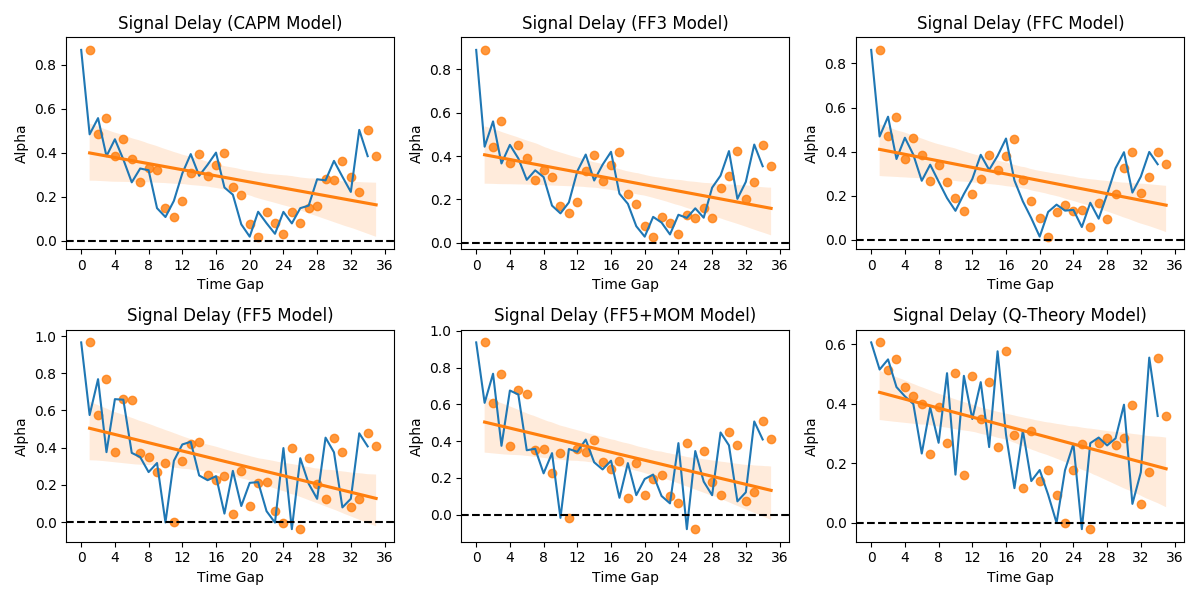
\includegraphics[width=\linewidth]{rfr_signal_delay.png}
    \caption{五组模型Q5-Q1结果(随机森林)}
    \label{signal1}
\end{figure}

\begin{figure}[htbp]
  \centering
    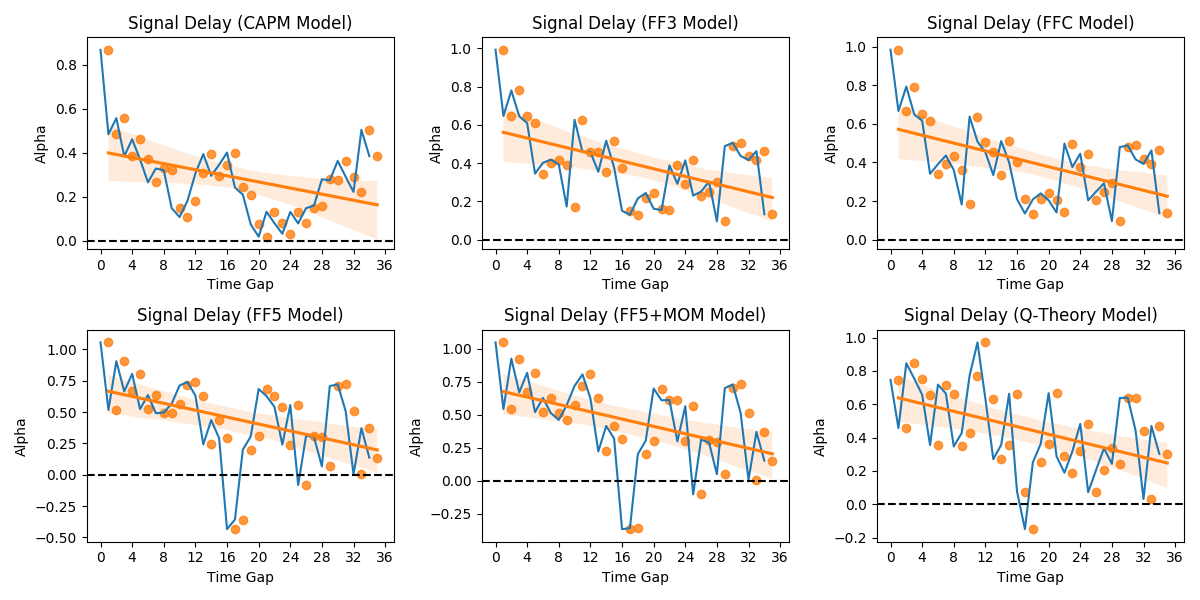
\includegraphics[width=\linewidth]{gbr_signal_delay.png}
    \caption{五组模型Q5-Q1结果(GBDT)}
    \label{signal2}
\end{figure}

在五组模型中,多空组合收益均在当前时点$t$拥有最高的超额收益$\alpha$,但后面随着时间增长,收益呈现明显的下降趋势,说明当前时点的错误定价已经随着时间而归正,股票的市场价格能够灵活随着信息进行调整,进而逐渐趋近于内在价值,收益也就越来越小,证明了本文在每一期重新进行内在价值计算、根据错误定价因子M对公司进行分组的正确性。若采用过往时点的结果进行未来股票收益的分析,会产生一定的偏误,所以要做到信息的更新换代。
\begin{figure}[htbp]
  \centering
   \begin{subfigure}[b]{0.48\textwidth}
     \centering
    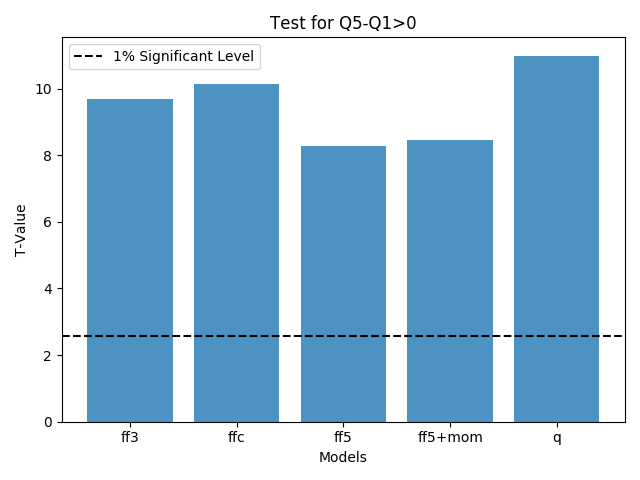
\includegraphics[width=\linewidth]{rfr_t_value.png}
    \caption{随机森林}
    \label{t1}
    \end{subfigure}
    \hfill
     \begin{subfigure}[b]{0.48\textwidth}
       \centering
    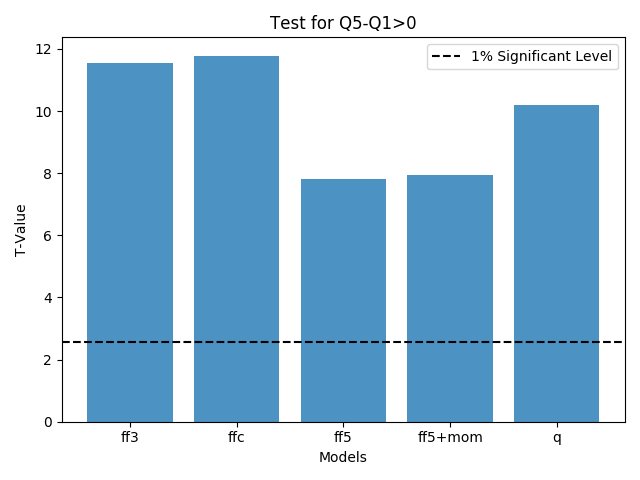
\includegraphics[width=\linewidth]{gbr_t_value.png}
    \caption{GBDT}
    \label{t2}
    \end{subfigure}
    \caption{五组模型多空组合显著性检验}
    \label{t}
\end{figure}

图~\ref{t}~是对于五组模型中多空组合收益是否显著大于0的检验,所有模型结果均在1\%的显著性水平下成立,证明了运用财务指标衡量公司内在价值的可行性、根据错误定价因子M进行公司分组的有效性。




%\subsection{原始代码}
%朴实的代码块:
%
%使用 verbatim 环境可以得到如下原样的输出。
%\begin{verbatim}
%print("Hello world!")
%\end{verbatim}
%
%使用 listings 包提供的 lstlisting 环境可以对代码进行进一步的格式化,minted 包所提供的 minted 环境还可以对代码进行高亮。更多定制功能请自行参照文档配置。
%
%\subsection{算法描述/伪代码}
%参考 \href{https://en.wikibooks.org/wiki/LaTeX/Algorithms}{Algorithms} 与 algorithm2e 文档,给出一个简单的示例,见算法 \ref{alg:alg1}。
%
%\begin{algorithm}
%  \SetAlgoLined
%  \KwData{this text}
%  \KwResult{how to write algorithm with \LaTeXe}
%  initialization\;
%  \While{not at end of this document}{
%    read current\;
%    \eIf{understand}{
%      go to next section\;
%      current section becomes this one\;
%    }{
%      go back to the beginning of current section\;
%    }
%  }
%  \caption{如何写算法}\label{alg:alg1}
%\end{algorithm}
%
%\section{绘图}
%关于使用 \LaTeX{} 绘图的更多例子,请参考 \href{https://www.overleaf.com/learn/latex/Pgfplots_package}{Pgfplots package}。一般建议使用如 Photoshop、PowerPoint 等制图,再转换成 PDF 等格式插入。
%
%\section{写在最后}
%工具不重要,对工具的合理运用才重要。希望本模板对大家的论文写作有所帮助。
